\section{Interférence}
\subsection{Cas général}
\subsubsection{Différence de marche}
\[\delta=\qty[\sum_in_id_i]_2-\qty[\sum_ini_di]_1+(p_2-p_1)\frac{\lambda_o}{2}+\frac{\lambda_o(\phi_2-\phi_1)}{2\pi}\]

\subsubsection{Intensité}
\[I=I_1+I_2+2\sqrt{I_1I_2}\cos{\theta}\cos(\psi_2-\psi_1) \]
\[(\psi_2-\psi_1)=k_o\delta=k_o(r_2-r_1)\]
% \[k_o=\frac{2\pi}{\lambda}\]


\subsection{Fentes de Young}
\begin{center}
    \includestandalone[width=.46\textwidth]{fig/young}
\end{center}
\begin{tabular}{ll}
    Constructive & \(\delta=m\lambda=d\sin{\theta}\)\\
    Destructive & \(\delta=(2m+1)\frac{\lambda}{2}=d\sin{\theta}\)\\[8pt]
    Dist. intensité & \(I=4I_o\cos^2\qty(\frac{k_o\delta}{2}) \)\\[8pt]
    Visibilité (Contraste) & \(V=\frac{2\sqrt{I_1I_2}}{I_1+I_2}\)
\end{tabular}



\subsection{Lames à faces parallèles (air-verre-air)}
\begin{center}
    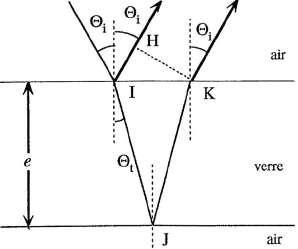
\includegraphics[height=.2\textwidth]{fig/parallel.PNG}
\end{center}
\begin{tabular}{ll}
    Différence de marche & \(\delta=2ne-\frac{\lambda_o}{2}\)\\
    Constructif & \(2e=(m+1/2)\frac{\lambda_o}{n}\) \\
    Destructif & \(2e=m\frac{\lambda_o}{n}\)
\end{tabular}

\subsection{Lames à faces presque parallèles (air-verre-air)}
\begin{center}
    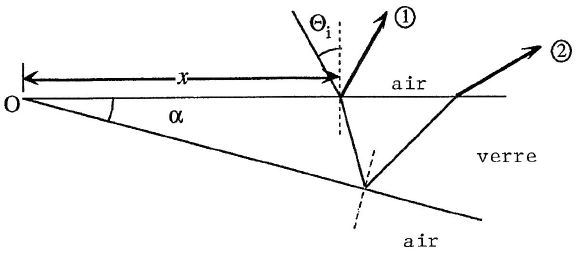
\includegraphics[width=0.35\textwidth]{fig/lames_presque_paralleles.PNG}    
\end{center}
% \vspace{-1\baselineskip}
\begin{tabular}{ll}
    Différence de marche & \(\delta=2ne-\frac{\lambda_o}{2}=2n\alpha x - \frac{\lambda_o}{2}\)\\[8pt]
    Constructif & \(x_c=(m+1/2)\frac{\lambda_o}{2\alpha n}\)\\[8pt]
    Destructif & \(x_d=\frac{m\lambda_o}{2\alpha n}\)\\[8pt]
    Dist. entrée-sortie & \(\Delta x = \frac{\lambda_o}{2\alpha n}\)
\end{tabular}


\subsection{Interféromètre de Michelson}
\begin{center}
    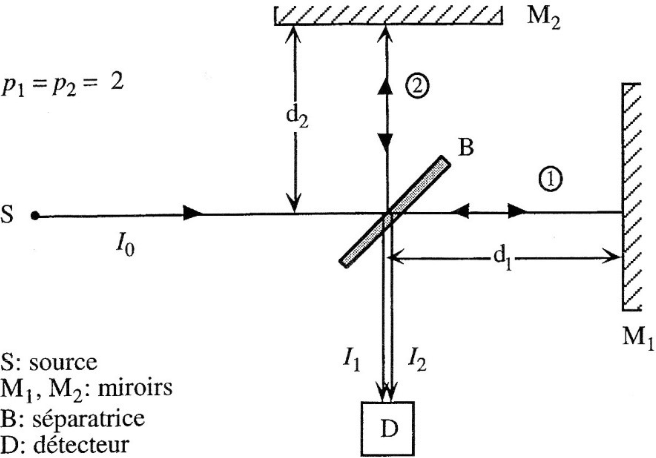
\includegraphics[width=.35\textwidth]{fig/michelson.png}
\end{center}
\begin{tabular}{ll}
    Différence de marche & \(\delta=2(d_2-d_1)\)\\
    Constructif & \(2(d_2-d_1)=m\lambda_o\) \\
    Destructif & \(2(d_2-d_1)=(2m+1)\frac{\lambda_o}{2}\)
\end{tabular}